% !TeX TXS-program:compile = txs:///lualatex

\documentclass[a4paper,11pt]{article}
\usepackage[revgoku]{cp-base}
\graphicspath{{./graphics/}}
%variables
\donnees[%
classe={1\up*{ère} 2M2},matiere={[SPÉ.MATHS]},mois=Janvier,annee=2022,typedoc=CHAP,numdoc=6
]
%formatage
\author{Pierquet}
\title{\nomfichier}
\hypersetup{pdfauthor={Pierquet},pdftitle={\nomfichier},allbordercolors=white,pdfborder=0 0 0,pdfstartview=FitH}
%divers
\lhead{\entete{\matiere}}
\chead{\entete{\lycee}}
\rhead{\entete{\classe{} - \mois{} \annee}}
\lfoot{\pied{\matiere}}
\cfoot{\logolycee{}}
\rfoot{\pied{\numeropagetot}}

\begin{document}

\ifdef{\cercletrigo}{}{%
	\newcommand\cercletrigo{%
		\draw (0,0) circle[radius=2] ;
		\draw (-2.25,0) -- (2.25,0) ;
		\draw (0,-2.25) -- (0,2.25) ;
		\draw[->,>=stealth'] (0,0) -- (2,0) ;
		\draw[->,>=stealth'] (0,0) -- (0,2) ;
		\draw (0,0) node[below left] {$O$} ;}
}

\ifdef{\angl}{}{\newcommand\angl[2]{\dfrac{#1\pi}{#2}}}

\pagestyle{fancy}

\part{CH06 - Trigonométrie - Exercices (Correction)}

\medskip

\exonum{0}%exon1

\medskip

On convertit en utilisant la proportionnalité $\ang{180} \leftrightarrow \pi^{r}$.
\begin{enumerate}
	\item $\ang{10}=\dfrac{\pi}{18}^{r} \approx 0,175^{r} \: ; \: \ang{59} \approx 1,030^{r} \: ; \: \ang{180}=\pi^{r} \: ; \: \ang{18}=\dfrac{\pi}{10}^{r} \: ; \: \ang{72}=\dfrac{2\pi}{5}^{r}\approx 1,257^{r} \: ; \: \ang{112,5}\approx 1,963^{r}$.
	\item $\dfrac{\pi}{3}=\ang{60} \: ; \: \dfrac{2\pi}{3}=\ang{120} \: ; \: \pi=\ang{180} \: ; \: \dfrac{5\pi}{4}=\ang{225} \: ; \: \dfrac{3\pi}{8}=\ang{67,5} \: ; \: \dfrac{5\pi}{12}=\ang{75} \: ; \: \dfrac{3\pi}{2}=\ang{270}$.
\end{enumerate}

\medskip

\exonum{1}%exon2

\medskip

On utilise le cercle trigo et le \og découpage en parts de pizza \fg{} :

\begin{center}
	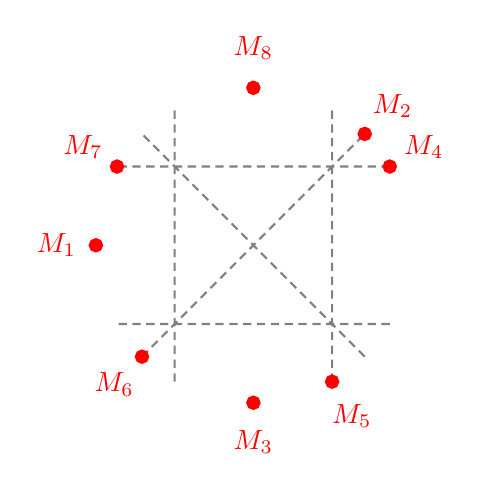
\begin{tikzpicture}[scale=1,very thick]
		\cercletrigo
		\draw[densely dashed, gray,thick] (-45:2) -- (135:2) (-135:2) -- (45:2) (30:2) -- (150:2) (-30:2) -- (-150:2) (-60:2)--(60:2) (-120:2)--(120:2) ;
		\foreach \angle/\numero in {180/1,45/2,270/3,30/4,-60/5,-135/6,150/7,-270/8}{
			\filldraw[red] (\angle:2) circle[radius=2pt] (\angle:2.5) node[red] {$M_{\numero}$} ;} 
	\end{tikzpicture}
\end{center}

\medskip

\exonum{2}%exon3

\medskip

On utilise le cercle trigo, en faisant attention à l'\textit{intervalle d'étude} :

\begin{enumerate}
	\item Pour M : on repère \og $\cos=0,5$ et en haut \fg, ce qui donne $\dfrac{\pi}{3}$ $\checkmark$
	
	Pour N : on repère \og $\cos=\pm\sin$ et en haut à gauche \fg, ce qui donne $\dfrac{3\pi}{4}$ $\checkmark$
	
	Pour P, on repère \og $\cos=0,5$ et en bas \fg, ce qui donne $\dfrac{-\pi}{3}$ ou ici $\dfrac{-\pi}{3}+2\pi=\dfrac{5\pi}{3}$ $\checkmark$
	\item Pour Q : on repère \og $\cos=\sin$ et en haut à droite \fg, ce qui donne $\dfrac{\pi}{4}$ $\checkmark$
	
	Pour R : on repère \og $\sin=-0,5$ et à gauche \fg, ce qui donne $\dfrac{-5\pi}{6}$ $\checkmark$
	
	Pour S, on repère \og $\sin=-0,5$ et à droite \fg, ce qui donne $\dfrac{-\pi}{6}$ $\checkmark$
\end{enumerate}

\medskip

\exonum{1}%exon4

\medskip

On réduit, à l'aide de la calculatrice, les résultats sont (bien évidemment) à $2\pi$ près (!) :
\begin{multicols}{3}
	\begin{enumerate}
		\item $\alpha=\angl{7}{2}=-\angl{}{2}$
		\item $\alpha=-\angl{4}{3}=\angl{2}{3}$
		\item $\alpha=\angl{35}{6}=-\angl{}{6}$
		\item $\alpha=-\angl{21}{4}=\angl{3}{4}$
		\item $\alpha=\angl{202}{3}=-\angl{2}{3}$
	\end{enumerate}
\end{multicols}

\newpage

\exonum{2}%exon5

\newcommand\ractd{\dfrac{\sqrt{3}}{2}}
\newcommand\ud{\dfrac{1}{2}}
\newcommand\racdd{\dfrac{\sqrt{2}}{2}}
\newcommand\angmpcossin[5][]{%
	\tabto{2cm}$\Rightarrow MP=#1\angl{#2}{#3}$ \tabto{4.5cm}et donc $\cos(\alpha)=#4$ \tabto{8.5cm}et $\sin(\alpha)=#5$
}

\begin{enumerate}
	\item $\alpha=\vphantom{\angl{1}{2}}\angl{}{6}$ \angmpcossin[]{}{6}{\ractd}{\ud} ;
	\item $\alpha=\angl{5}{6}$ \angmpcossin[]{5}{6}{-\ractd}{\ud} ;
	\item $\alpha=\angl{7}{6}$ \angmpcossin[-]{5}{6}{-\ractd}{-\ud} ;
	\item $\alpha=\angl{11}{6}$ \angmpcossin[-]{}{6}{\ractd}{-\ud} ;
	\item $\alpha=\angl{13}{6}$ \angmpcossin[]{}{6}{\ractd}{\ud} ;
	\item $\alpha=\vphantom{\angl{1}{2}}\angl{}{4}$ \angmpcossin[]{}{4}{\racdd}{\racdd} ;
	\item $\alpha=\angl{9}{4}$ \angmpcossin[]{}{4}{\racdd}{\racdd} ;
	\item $\alpha=\angl{5}{4}$ \angmpcossin[-]{3}{4}{-\racdd}{-\racdd} ;
	\item $\alpha=\angl{81}{4}$ \angmpcossin[]{}{4}{\racdd}{\racdd} ;
	\item $\alpha=-\angl{108}{4}$ \tabto{2cm}$\Rightarrow MP=-\pi$ \tabto{4.5cm}et donc $\cos(\alpha)=-1$ \tabto{8.5cm}et $\sin(\alpha)=0$ ;
	\item $\alpha=\angl{4}{3}$ \angmpcossin[-]{2}{3}{-\ud}{-\ractd} ;
	\item $\alpha=\vphantom{\angl{1}{2}}\angl{}{3}$ \angmpcossin[]{}{3}{\ud}{\ractd} ;
	\item $\alpha=\angl{71}{3}$ \angmpcossin[-]{}{3}{\ud}{-\ractd} ;
	\item $\alpha=\angl{97}{3}$ \angmpcossin[]{}{3}{\ud}{\ractd} ;
	\item $\alpha=-\angl{54}{3}$ \tabto{2cm}$\Rightarrow MP=0$ \tabto{4.5cm}et donc $\cos(\alpha)=1$ \tabto{8.5cm}et $\sin(\alpha)=0$.
\end{enumerate}

\medskip

\exonum{2}%exon6

\medskip

On va placer les angles (à l'aide de la mesure principale) \og bornes \fg{} des intervalles et parcourir le cercle :

\begin{itemize}
	\item $\red \mathscr{I}=\intervFF{-\dfrac{\pi}{4}}{0} \cup \intervFF{0}{\dfrac{5\pi}{4}} = \intervFF{\textcircled{1}}{\textcircled{2}} \cup \intervFF{\textcircled{2}}{\textcircled{3}}$ ;
	\item $\blue \mathscr{J}=\intervFF{\dfrac{4\pi}{3}}{2\pi} \cup \intervFF{2\pi}{\dfrac{13\pi}{6}} = \intervFF{\textcircled{1}}{\textcircled{2}} \cup \intervFF{\textcircled{2}}{\textcircled{3}}$ ;
	\item $\green \mathscr{K}=\intervFF{\dfrac{-7\pi}{6}}{0} \cup \intervFF{0}{\dfrac{5\pi}{4}} = \intervFF{\textcircled{1}}{\textcircled{2}} \cup \intervFF{\textcircled{2}}{\textcircled{3}}$.
\end{itemize}

\begin{center}
	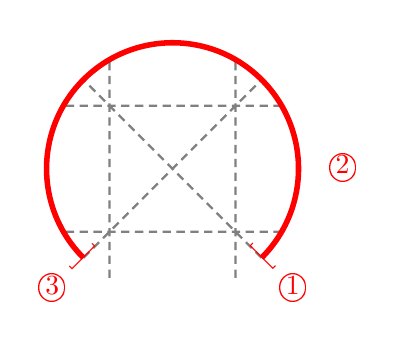
\begin{tikzpicture}[very thick,scale=0.8]
		\cercletrigo
		\draw[densely dashed, gray,thick] (-45:2) -- (135:2) (-135:2) -- (45:2) (30:2) -- (150:2) (-30:2) -- (-150:2) (-60:2)--(60:2) (-120:2)--(120:2) ;
		\draw (-45:2) node[red,rotate=45] {\large$\boldsymbol{\big[}$} ;
		\draw (-135:2) node[red,rotate=-45] {\large$\boldsymbol{\big]}$} ;
		\draw[line width=2pt,red] (-45:2) arc(-45:225:2) ;
		\draw (-45:2.7) node[red] {\textcircled{1}} ;
		\draw (0:2.7) node[red] {\textcircled{2}} ;
		\draw (-135:2.7) node[red] {\textcircled{3}} ;
	\end{tikzpicture}
	\qquad \qquad
	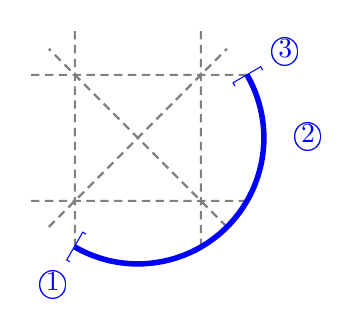
\begin{tikzpicture}[very thick,scale=0.8]
		\cercletrigo
		\draw[densely dashed, gray,thick] (-45:2) -- (135:2) (-135:2) -- (45:2) (30:2) -- (150:2) (-30:2) -- (-150:2) (-60:2)--(60:2) (-120:2)--(120:2) ;
		\draw (-120:2) node[blue,rotate=-30] {\large$\boldsymbol{\big[}$} ;
		\draw (30:2) node[blue,rotate=-60] {\large$\boldsymbol{\big[}$} ;
		\draw[line width=2pt,blue] (-120:2) arc(-120:30:2) ;
		\draw (-120:2.7) node[blue] {\textcircled{1}} ;
		\draw (0:2.7) node[blue] {\textcircled{2}} ;
		\draw (30:2.7) node[blue] {\textcircled{3}} ;
	\end{tikzpicture}
	\qquad \qquad
	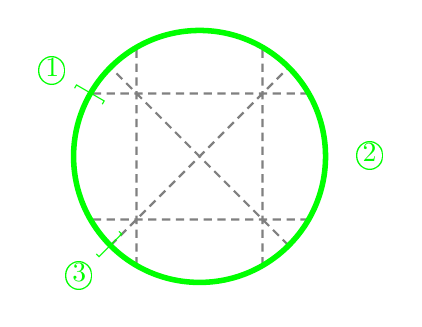
\begin{tikzpicture}[very thick,scale=0.8]
		\cercletrigo
		\draw[densely dashed, gray,thick] (-45:2) -- (135:2) (-135:2) -- (45:2) (30:2) -- (150:2) (-30:2) -- (-150:2) (-60:2)--(60:2) (-120:2)--(120:2) ;
		\draw (-135:2) node[green,rotate=-45] {\large$\boldsymbol{\big]}$} ;
		\draw (150:2) node[green,rotate=60] {\large$\boldsymbol{\big]}$} ;
		\draw[line width=2pt,green] (0,0) circle[radius=2] ;
		\draw (150:2.7) node[green] {\textcircled{1}} ;
		\draw (0:2.7) node[green] {\textcircled{2}} ;
		\draw (-135:2.7) node[green] {\textcircled{3}} ;
	\end{tikzpicture}
\end{center}

\medskip

\exonum{2}%exon7

\medskip

On utilise le cercle trigo pour \og lire \fg{} les solutions :

\begin{enumerate}
	\item \textcolor{purple}{$\cos(x)=\dfrac{\sqrt{2}}{2}$} :%
	\tabto{4cm}
	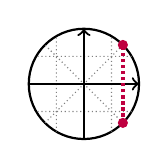
\begin{tikzpicture}[thick,scale=0.7,baseline=(current bounding box.center)]
		\draw (0,0) circle[radius=1] ;
		\draw[densely dotted, gray,thin] (-45:1) -- (135:1) (-135:1) -- (45:1) (30:1) -- (150:1) (-30:1) -- (-150:1) (-60:1)--(60:1) (-120:1)--(120:1) ;
		\draw[->] (0,-1)--(0,1) ; \draw[->] (-1,0)--(1,0) ;
		\draw[purple,densely dotted,very thick] (-45:1)--(45:1) ;
		\filldraw[purple] (-45:1) circle[radius=2pt] (45:1) circle[radius=2pt] ;
	\end{tikzpicture}%
	\tabto{6.5cm}
	 $\mathscr{S}=\begin{dcases} x = \dfrac{\pi}{4}+2k\pi \\ x = -\dfrac{\pi}{4}+2k\pi \end{dcases}$ avec $k$ entier.%
	\item {\blue $\sin(x)=0\vphantom{\dfrac{\sqrt{2}}{2}}$} : %
	\tabto{4cm}
	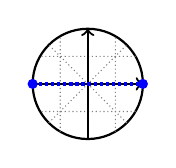
\begin{tikzpicture}[thick,scale=0.7,baseline=(current bounding box.center)]
		\draw (0,0) circle[radius=1] ;
		\draw[densely dotted, gray,thin] (-45:1) -- (135:1) (-135:1) -- (45:1) (30:1) -- (150:1) (-30:1) -- (-150:1) (-60:1)--(60:1) (-120:1)--(120:1) ;
		\draw[->] (0,-1)--(0,1) ; \draw[->] (-1,0)--(1,0) ;
		\draw[blue,densely dotted,very thick] (180:1)--(0:1) ;
		\filldraw[blue] (180:1) circle[radius=2pt] (0:1) circle[radius=2pt] ;
	\end{tikzpicture}%
	\tabto{6.5cm}$\mathscr{S}=\begin{dcases} x = 0+2k\pi \\ x = \pi+2k\pi \end{dcases}$ avec $k$ entier.
	\item $2\sin(x)+\sqrt{3}=0 \ssi {\red \sin(x)=-\dfrac{\sqrt{3}}{2}}$ :%
	\tabto{7cm}
	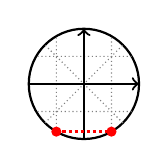
\begin{tikzpicture}[thick,scale=0.7,baseline=(current bounding box.center)]
		\draw (0,0) circle[radius=1] ;
		\draw[densely dotted, gray,thin] (-45:1) -- (135:1) (-135:1) -- (45:1) (30:1) -- (150:1) (-30:1) -- (-150:1) (-60:1)--(60:1) (-120:1)--(120:1) ;
		\draw[->] (0,-1)--(0,1) ; \draw[->] (-1,0)--(1,0) ;
		\draw[red,densely dotted,very thick] (-120:1)--(-60:1) ;
		\filldraw[red] (-120:1) circle[radius=2pt] (-60:1) circle[radius=2pt] ;
	\end{tikzpicture}%
	\tabto{9.5cm}
	$\mathscr{S}=\begin{dcases} x = -\dfrac{\pi}{3}+2k\pi \\ x = -\dfrac{2\pi}{3}+2k\pi \end{dcases}$ avec $k$ entier. 
\end{enumerate}

\medskip

\exonum{3}%exon8

\begin{enumerate}
	\item 
	\begin{enumerate}
		\item $\sin(x)=\dfrac23 \Rightarrow \sin^2(x)=1-\left(\dfrac23\right)^2=\dfrac59$ et $x \in \intervFF{0}{\dfrac{\pi}{2}}$, donc $\sin(x)\pg 0$ et $\sin(x)=\sqrt{\dfrac59}=\dfrac{\sqrt{5}}{3}$.
		\item $\cos(x)=-\dfrac15 \Rightarrow \sin^2(x)=1-\left(-\dfrac15\right)^2=\dfrac{24}{25}$ et $x \in \intervFF{-\pi}{0}$, donc $\sin(x) \pp0$ et  $\sin(x)=-\sqrt{\dfrac{24}{25}}=-\dfrac{2\sqrt{6}}{5}$.
		\item $\sin(x)=-\dfrac{\sqrt{5}}{3} \Rightarrow \cos^2(x)=1-\left(-\dfrac{\sqrt{5}}{3}\right)^2=\dfrac49$ et $x \in \intervFF{\dfrac{\pi}{2}}{\pi}$, donc $\cos(x) \pp0$ et $\cos(x)=-\sqrt{\dfrac49} = -\dfrac23$.
	\end{enumerate}
	\item On va développer :
	\begin{enumerate}
		\item $\big(\cos(x) + \sin(x)\big)^2 + \big(\cos(x) - \sin(x)\big)^2$
		
		\hspace{1cm}$=\cos^2(x)+2\cos(x)\sin(x)+\sin^2(x)+\cos^2(x)-2\cos(x)\sin(x)+\sin^2(x) = 2\cos^2(x)+2\sin^2(x) = 2$ ;
		\item $\big(\cos(x) + \sin(x)\big)^2 - \big(\cos(x) - \sin(x)\big)^2$
		
		\hspace{1cm}$=\cos^2(x)+2\cos(x)\sin(x)+\sin^2(x)-\cos^2(x)+2\cos(x)\sin(x)-\sin^2(x) = 4\cos(x)\sin(x)$.
	\end{enumerate}
%	\item Exprimer à l’aide de $\sin(x)$ et $\cos(x)$, les expressions suivantes :
%	\begin{enumerate}
%		\item $\sin(-x) + \cos(-x) = -\sin(x) + \cos(x)$ ;
%		\item $\sin(-x) - \sin(\pi +x) = -\sin(x) + \sin(x) = 0$ ;
%		\item $\sin(-x) + \cos(-x) = -\sin(x) + \cos(x)$ ;
%		\item $\sin\left(x+\angl{}{2}\right) - 3\cos \left(-\angl{}{2} - x \right) - 4 \sin(\pi-x) = \cos(x) + 3\sin(x)-4\sin(x)=\cos(x)-\sin(x)$.
%	\end{enumerate}
\end{enumerate}

\medskip

\exonum{4}%exon9

\begin{enumerate}
	\item $2\sin \left(x+\angl{}{4}\right)-1 = 0 \ssi \sin \left(x+\angl{}{4}\right)=\dfrac12$  ; ainsi $\mathscr{S}=\begin{dcases} x+\angl{}{4} = \dfrac{\pi}{6}+2k\pi \\ x+\angl{}{4} = \dfrac{5\pi}{6}+2k\pi \end{dcases} = \begin{dcases} x = -\dfrac{\pi}{12}+2k\pi \\ x = \dfrac{7\pi}{12}+2k\pi \end{dcases}$ avec $k$ entier.
	\item $1-\sqrt{2} \cos \left(\angl{}{3} - x \right) = 0 \ssi \cos \left(\angl{}{3} - x \right)=\dfrac{1}{\sqrt{2}}=\racdd$ ;
	
	\hspace{1cm}ainsi $\mathscr{S}=\begin{dcases} \angl{}{3} - x = \dfrac{\pi}{4}+2k\pi \\ \angl{}{3} - x = -\dfrac{\pi}{4}+2k\pi \end{dcases} = \begin{dcases} x = \dfrac{\pi}{12}-2k\pi \\ x = \dfrac{7\pi}{12}-2k\pi \end{dcases}$ avec $k$ entier ;
	\item $\sin \left(2x - \angl{}{4} \right) = \dfrac12$ ; ainsi $\mathscr{S}=\begin{dcases} 2x - \angl{}{4} = \dfrac{\pi}{6}+2k\pi \\ 2x - \angl{}{4} = \dfrac{5\pi}{6}+2k\pi \end{dcases} = \begin{dcases} x = \dfrac{5\pi}{24}+k\pi \\ x = \dfrac{13\pi}{24}+k\pi \end{dcases}$ avec $k$ entier ;
	\item $\cos \left(2x -\angl{}{3} \right) = \dfrac12$ ; ainsi $\mathscr{S}=\begin{dcases} 2x -\angl{}{3} = \dfrac{\pi}{3}+2k\pi \\ 2x -\angl{}{3} = -\dfrac{\pi}{3}+2k\pi \end{dcases} = \begin{dcases} x = \dfrac{\pi}{3}+k\pi \\ x = 0+k\pi \end{dcases}$ avec $k$ entier.
\end{enumerate}

\end{document}